\section{Study 1: Acquiring, retaining, and reconsidering evidence}
\label{sec:study}
\subsection{Research questions and organizational instance}
Study 1 follows a change from its discovery to its later use. It asks whether evidence retention alters the value of evaluator revision, whether a one-time discovery can substitute for repeated search, and which part of reassessment produces a measured gain. These questions instantiate $U.a$ (evidence acquisition), $M$ (retained evidence), and $U.r$ (continued use or reconsideration) in the specification.

The relations in \cref{tab:obligations} constrain specific design decisions. Decision--memory requires separate records for workflow labels, program scores, and the adopted program; we therefore intervene on these memories separately. Cost--resource requires each queried label to enter one ledger, even when both program trials and workflow selection reuse it. Actor--evidence requires current program trials to share the same pre-review information and prevents access to hidden error probabilities. Outcome--criterion keeps the deployment horizon and net-value rule common across arms. Study 1 uses these obligations to distinguish a change in the evaluator from a change in its evidence.

A proposer supplies three workflow templates, an evaluator acquires labels, and a review board may replace the evaluation program. In Study 1, the roles denote information access and decision rights and can be assigned to humans or agents; Study 2 models their individual judgments (Section~\ref{sec:actor-review}). The environment has two equally frequent observable task strata. Error probabilities are $(.20,.20)$ for the standard template, $(.16,.16)$ for broad, and initially $(.08,.46)$ for specialized. Thus broad is initially best, while specialized helps one stratum and harms the population. In \emph{stationary harm} these probabilities remain fixed. In \emph{workflow reversal}, specialized becomes $(.08,.08)$ before round 25 and becomes the best template. \emph{Uniform gain} uses that improving specialized template throughout. The probabilities define synthetic mechanism contrasts, not fitted organizational parameters.

Each of 48 rounds deploys one template on 4096 production tasks. Only acquired evaluation labels enter decisions; the external scorer uses exact expected production outcomes. This separates uncertainty in organizational judgment from production sampling noise. One value unit is the gross value assigned to one completed production task before errors and costs. Net value per task subtracts error penalties and modeled expenses in these normalized units. An error costs 3 units, generation costs $.02$ per production or evaluation output, a label costs $.20$, and changing evaluation programs costs $.50$. Storage and computation costs are outside this ledger.

\subsection{Memory and decision rules}
The population-weighted posterior error estimate of template $k$ is
\begin{equation}
\widehat r_{k,t}=\frac12\sum_{s=1}^{2}\frac{1+E_{ks,t}}{2+N_{ks,t}},
\label{eq:risk}
\end{equation}
where $E$ and $N$ count observed errors and labels available to the decision. All conditions begin with $\operatorname{Beta}(1,1)$. \emph{Reset} uses current-round evidence only. \emph{Cumulative} retains all earlier evidence. \emph{Window 8} retains evidence from the preceding eight rounds plus current observations. The same retention rule applies to past evaluation-program scores; a program's identity remains retained until another is selected. This separates remembering a decision from remembering the evidence supporting it.

Three evaluation programs form a fixed catalog. Biased allocates 95\% of a template's allowance to the first stratum. Balanced uses equal counts. Neyman uses a two-label-per-cell pilot and posterior variance estimates to allocate the remainder across strata \citep{neyman}. Each program chooses the template minimizing \cref{eq:risk}. Counts use population weights regardless of sampling proportions.

Workflow selection is a fixed-budget identification problem: evaluation outputs are acquired to choose a template for subsequent deployment. Successive Rejects addresses this objective by progressively eliminating candidates \citep{bai}; exploration sampling explicitly targets policy choice rather than immediate experimental outcomes \citep{kasy}. We use a between-template elimination comparator based on successive rejection, whereas Neyman allocates within each template. It observes paired stratum labels, eliminates the worst estimated candidate after a first phase, and compares the remaining two after a second phase. Historical evidence enters the same estimates under the memory conditions; this is a memory-augmented implementation of the rejection schedule, with no claim to transfer stationary theoretical guarantees to the reversal environment. Allocation formulas and tie rules appear in Appendix~\ref{app:protocol}.

\subsection{Discovery, reuse, and fixed resource ceilings}
\Cref{tab:arms} distinguishes knowing an evaluator, discovering it once, and periodically reconsidering it. A label unit is one observed binary error outcome for one evaluated output. Every arm receives a ceiling of 2736 such observations per eight-round block. A fixed arm can allocate 342 units per round, or 114 per template for the three catalog programs. Discover once pays for program comparisons only before round 1. Repeated discovery compares programs before rounds 1, 9, 17, 25, 33, and 41. Both begin with Biased and select among the same catalog.

\begin{table}[t]
\caption{Decision rules and the comparisons they support. All arms use the same memory condition and block-level resource ceiling.}
\label{tab:arms}\small
\begin{tabularx}{\linewidth}{@{}p{.23\linewidth}YY@{}}\toprule
Arm & Program decision & Role in the study \\\midrule
Biased / Balanced / Neyman & Program specified before execution & Fixed designs with different coverage/allocation rules. \\
Successive rejection & Fixed elimination rule across templates & A between-template elimination comparator. \\
Discover once & Compare programs once; retain the winner & Discovery followed by reuse and budget reallocation. \\
Repeated discovery & Reassess every eight rounds & Incremental value of continued program assessment. \\
Trial-matched Balanced & Run the same trials; keep Balanced & Exploratory control for evidence acquisition and timing. \\\bottomrule
\end{tabularx}
\end{table}

In the base design, program trials receive at most 20\% of the block ceiling, with one trial per catalog program. Each trial screens the three workflows under the same pre-review memory snapshot, selects one, and validates it on fresh balanced labels. Its score is validation value less screening expense per production task. The highest mean retained trial score determines the program. This fixed outer selector implements bounded program revision. It does not generate new algorithms.

All acquired trial labels, including evidence from rejected programs, can enter workflow memory exactly once. Decisions about program scores precede pooling the current trials; the subsequent operational screen receives the pooled evidence. This makes failed searches potential sources of reusable information. Actual trial expenditure is deducted from the current block, and the remaining allowance is spread across its operational screens. Discover once receives the full operational allowance from block 2 onward. No arm borrows from a future block; unused units due to integer allocation are not charged.

Net value includes production generation, all acquired labels, all evaluated outputs, and program changes. Selection regret measures the gross value gap to the best available template, separately from those costs. Harmful adoption counts choices worse than standard; after reversal, this measure becomes zero for all templates, so regret and adaptation trajectories are needed to distinguish them. The primary outcome averages net value over all 48 rounds, with final-eight-round performance as a separate endpoint.

The core matrix crosses three environments, three memory rules, and six arms, using 128 independent replicate streams per cell. A separate 96-replicate grid crosses program-budget shares $.2,.4,.6$ with trial counts $1,3,6$, keeping the total ceiling fixed. It also removes program-score memory or trial-label pooling separately. After inspecting the core results, we added an explicitly exploratory trial-matched control and reversals before rounds 21 and 29 on new streams, to test attribution and timing. Appendix~\ref{app:protocol} specifies all conditions. Supplementary Tables S1--S5, supplied as the arXiv ancillary file \texttt{supplementary\_tables.pdf}, report Monte Carlo intervals and secondary outcomes for all conditions across the two studies and audit controls; conditional program groups in S2 are descriptive summaries without intervals. Each table identifies its repository source.

\subsection{Accumulation changes the apparent cost of improvement}
\Cref{fig:memory} reports every core arm and memory condition. Under stationary harm, cumulative evidence raises Balanced's mean net value from $.45224$ to $.48007$, a paired gain of $.02783$ (95\% Monte Carlo interval $.02659$--$.02907$). Its final-eight-round value reaches $.48163$, the value of consistently selecting broad under its actual evaluation expenditure. Balanced's mean selection regret falls from $.02939$ to $.00156$ per task, while its evaluation expense remains $.01837$. The net-value gain therefore equals the reduction in selection regret.

\begin{figure}[t]
\centering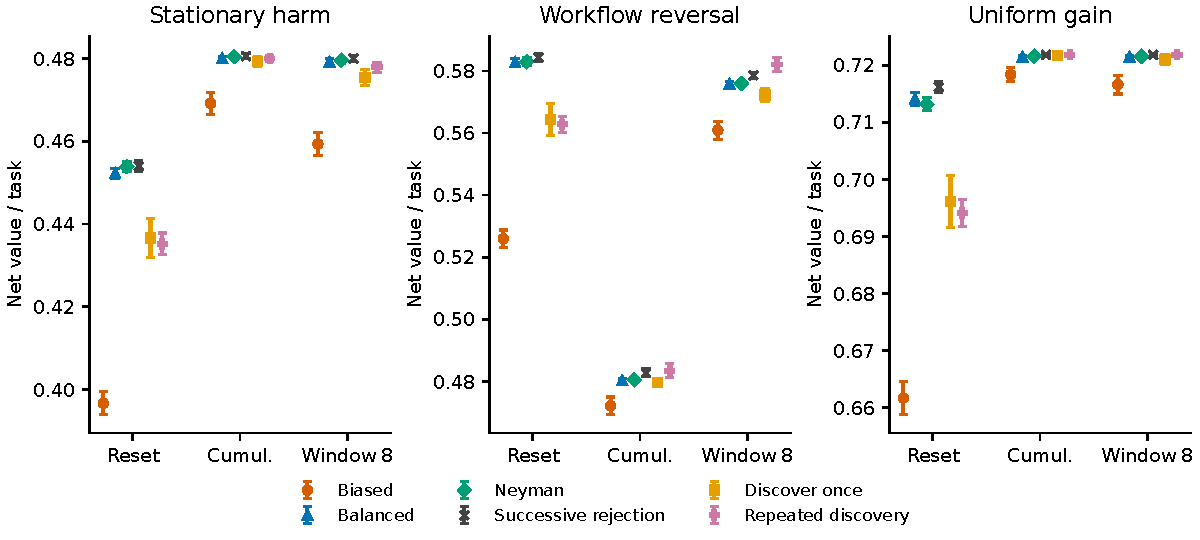
\includegraphics[width=\linewidth]{figures/fig9_memory.pdf}
\caption{All core comparisons: 128 replicate trajectories per cell, means and 95\% Monte Carlo intervals. Each panel uses its own value scale. ``Cumul.'' retains all acquired evidence; Window 8 retains the preceding eight rounds plus current evidence. The results concern the jointly specified memory, discovery, and acquisition rules.}
\label{fig:memory}
\end{figure}

Repeated discovery is $.01702$ below Balanced with reset evidence (interval $-.01964$ to $-.01440$). With cumulative evidence, that difference becomes $-.00007$ (interval $-.00100$ to $.00085$). Discover once reaches $.47928$, and repeated discovery $.48000$. Thus the sizeable reset disadvantage does not persist when paid-for evidence is reused. This does not establish equivalence: Study 1 estimates a small difference with the stated uncertainty. Successive rejection reaches $.48059$ under cumulative evidence, providing a competitive fixed selection rule. Across the nine environment--memory cells, successive rejection has the largest unrounded core mean in five. In the two retained-memory Uniform gain cells, its mean is less than $.00004$ below repeated discovery. These are descriptive rankings, not tests of equivalence. Under Uniform gain, specialized is best from the outset, so retention improves selection without the obsolescence cost seen after reversal; a fixed elimination rule remains competitive without program replacement.

The comparison to fixed programs also depends on prior knowledge. An equal-probability initial draw from the three catalog programs defines an ex ante fixed-program mixture, computed as their average conditional value. Under stationary harm, its net values are $.43426$ with reset evidence and $.47657$ with cumulative evidence. Repeated discovery exceeds these prior-averaged references by $.00096$ and $.00343$, respectively. Table~\ref{tab:base} reports the mixture in every core condition. Balanced is a prespecified representative-sampling rule, not an ex post oracle. These comparisons distinguish the cost of discovering a program from the value of revising an already reasonable design.

\subsection{Evidence can become obsolete before an organization forgets it}
Under workflow reversal, indefinite accumulation slows the replacement of broad by the newly superior specialized template. Balanced's full-horizon values are $.48026$ with cumulative memory, $.57583$ with Window 8, and $.58280$ with reset evidence. The finite window improves considerably on unlimited accumulation, yet its transition delay makes it worse than reset over this particular horizon. In the final eight rounds it reaches $.72163$, compared with $.71237$ for reset and $.48280$ for cumulative memory. \Cref{fig:attribution}a displays the corresponding deployment choices.

\begin{figure}[t]
\centering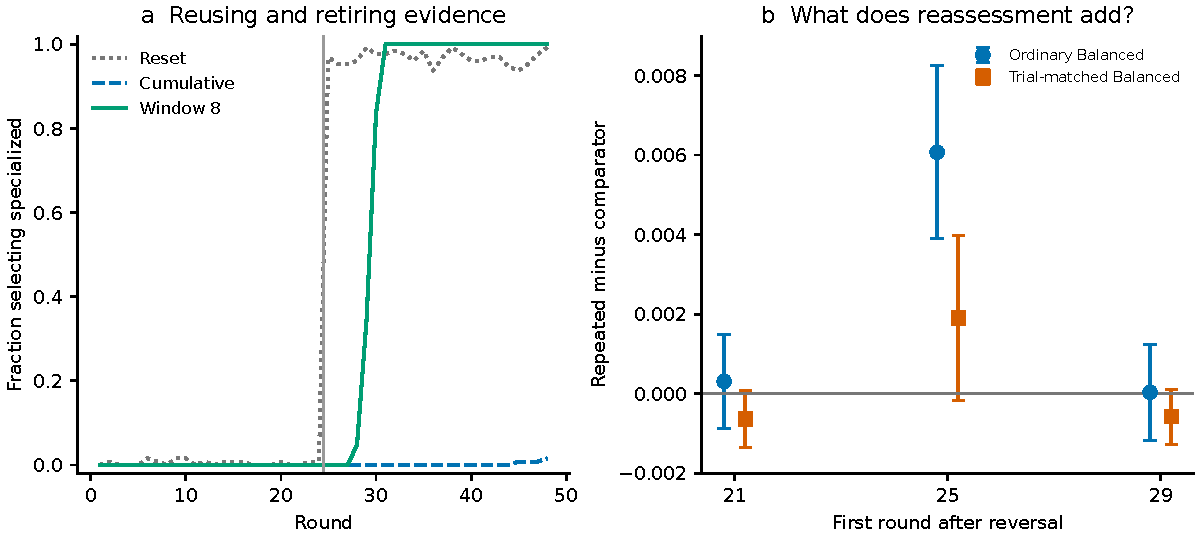
\includegraphics[width=\linewidth]{figures/fig10_attribution.pdf}
\caption{Retention and attribution. (a) Fixed Balanced under the core reversal; the vertical line marks the change before round 25. (b) Exploratory controls with Window 8 and reversals before rounds 21, 25, or 29. Points show repeated-discovery minus comparator differences with paired 95\% Monte Carlo intervals on 128 fresh replicate streams. Matching the trials, label reuse, and timing changes the attribution of the apparent reassessment gain.}
\label{fig:attribution}
\end{figure}

With Window 8 in the core reversal, repeated discovery exceeds discover-once by $.00975$ (interval $.00709$--$.01242$) and ordinary Balanced by $.00623$. These differences include the effects of concentrated trial acquisition and pooling, as well as the possibility of replacing the program. On the fresh exploratory streams, reversal before round 25 gives a repeated-discovery advantage of $.00607$ over ordinary Balanced (interval $.00390$--$.00825$). Matching program trials and label reuse while keeping Balanced reduces this difference to $.00191$ (interval $-.00016$ to $.00398$). For reversals before rounds 21 and 29, repeated discovery minus trial-matched Balanced is $-.00063$ and $-.00057$, respectively; both intervals span zero. The corresponding differences against ordinary Balanced are $.00031$ and $.00004$. The design therefore does not identify a stable gain from program replacement across the tested timings.

\subsection{What the allocation and retention diagnostics explain}
The full nine-cell budget-share/trial-count grid is reported in \cref{tab:grid}. More trial expenditure can improve the total repeated-discovery package when it also provides reusable workflow evidence. Consequently, ``meta-evaluation expenditure'' is not synonymous with discarded operational evidence. Removing trial-label pooling lowers repeated discovery from $.48043$ to $.47751$ under stationary cumulative memory, and from $.58214$ to $.57392$ under reversal with Window 8 on the independent sensitivity streams. Resetting only the program-score history has much smaller mean effects in these two conditions. These are interventions on different memory components, rather than interchangeable definitions of learning.

\Cref{tab:programs} reports retained-program proportions and subsequent-block outcomes conditional on retaining Balanced; Supplementary Table S2 reports all three retained programs and all three memory conditions for both discover-once and repeated-discovery rules across the three environments. At the last stationary review with cumulative memory, Biased, Balanced, and Neyman are retained in 38.3\%, 31.2\%, and 30.5\% of runs. The 40 runs retaining Balanced have subsequent-block net value $.4819$ and zero harmful adoption. Accurate workflow selection therefore need not coincide with convergence to one program when programs share a well-informed workflow memory. These summaries describe selection and downstream performance together; because retained programs are selected endogenously, their conditional means are not causal program effects. The combined evidence supports a narrower and more useful explanation of organizational improvement: gains depend on what the organization learns from evaluation, how long that evidence remains relevant, and whether a measured gain survives a control with the same information acquisition.
